\documentclass[11pt] {article}
\usepackage[]{graphicx}
\usepackage[]{color}
\usepackage[left=1in,right=1in,top=1in,bottom=1in,%
            footskip=.25in]{geometry}
\parskip=\smallskipamount
\parindent=0.0in

\begin{document}

Introduction to Data Science \\
Winter 2018

\bigskip

{\Large\bf Midterm Exam}

\bigskip

\begin{itemize}
\item You have 45 minutes to complete the exam

\item The exam is closed book, closed notes, closed computer, closed 
calculator, except one hand-written 8.5� $\times$ 11� crib sheet of your own creation and the official study guide provided with the exam.

\item Mark your answers {\bf on the exam itself}. We will {\bf not} grade answers written on scratch paper. If you run out of room, continue on the back of the page.
\end{itemize}

\rule{\textwidth}{1mm} %%==================================================

\medskip

{\large\bf Name}

\medskip

\rule{\textwidth}{1mm} %%==================================================

\medskip

{\large\bf Student id number}

\medskip

\rule{\textwidth}{1mm} %%==================================================

\medskip

{\large\bf Email}

\medskip

\rule{\textwidth}{1mm} %%==================================================

\medskip

{\large\bf All the work on this exam is my own}\\
(Please sign)

\medskip


\newpage %%%%%%%%%%

{\Large\bf Maternal smoking and pregnacies}

Printed below are the first three rows of a table. The column labels should be self explanatory.

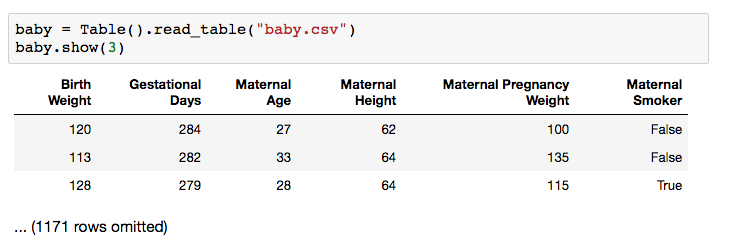
\includegraphics[width=15cm] {baby-table.png}

In the following you may assume that the statements {\bf \texttt from data science import $\star$} and \\ {\bf \texttt import numpy as np} have been executed.

\bigskip\bigskip

{\bf Problem 1} (10 points)

Write Python code that computes the birth weight of the heaviest baby.

\vspace{2cm}

\rule{\textwidth}{1mm} %%==================================================

{\bf Problem 2} (10 points)

Write Python code that computes the average birth weight of all babies.

\vspace{2cm}

\rule{\textwidth}{1mm} %%==================================================

{\bf Problem 3} (10 points)

Write Python code that computes the average birth weight of babies 
of 33 year old mothers.

\vspace{2cm}

\rule{\textwidth}{1mm} %%==================================================

{\bf Problem 4} (10 points)

Write Python code that computes the average birth weight of babies 
of 33 year old smokers.


\newpage %%%%%%%%%%

{\bf Problem 5} (10 points)

Write Python code that draws a bar chart showing the mean birth weights for babies of smokers and babies of non-smokers.

\vspace{2cm}

\rule{\textwidth}{1mm} %%==================================================

{\bf Problem 6} (20 points)

Write a function 

\hspace{1cm}{\texttt mean\_birth\_weight(query\_age)} 

that returns the average birth weight of babies with Maternal Age = query\_age if there are such babies in the data set, and "None" otherwise.

{\bf Hint:} Using \ \ {\bf\texttt Table.where}\ \  returns a table with 0 rows if there are no rows matching the predicate you supply.

\vspace{8cm}

\rule{\textwidth}{1mm} %%==================================================

{\bf Problem 7} (10 points)

The average birth weight for babies of smokers is 114oz, while the average birth weight for babies of non-smokers is 123oz. Based solely on this information, can you conclude that smoking causes low birth weight? Briefly justify your answer.


\newpage %%%%%%%%%%

{\bf Problem 8} (10 points)

In 1954 the Public Health Service conducted a study  to test the effectiveness of Jonas Salk's polio vaccine. The incidence of polio among children who were vaccinated was 28 per 100,000, while the incidence among unvaccinated children was 71 per 100,000. The Public Health Service concluded that the vaccine does indeed reduce the incidence of polio. What is the crucial aspect of the study that justifies this conclusion?

\vspace{2cm}

\rule{\textwidth}{1mm} %%==================================================\\

{\bf Problem 9} (5 points)

In the figure below, draw the conditional mean of Y, given X.

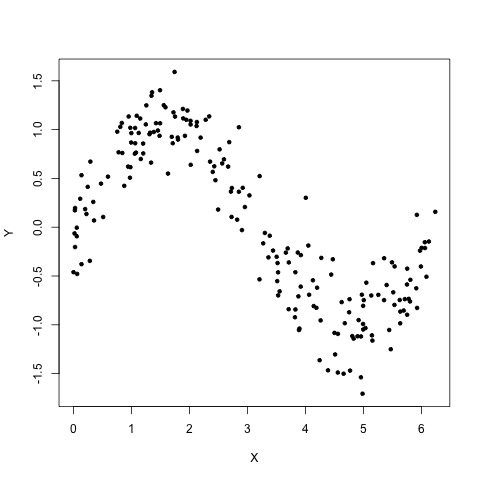
\includegraphics[height=7cm]{new-sin-wave.jpg}


\rule{\textwidth}{1mm} %%==================================================

{\bf Problem 10} (5 points)

In the figure below, draw the condition mean of Y, given X.

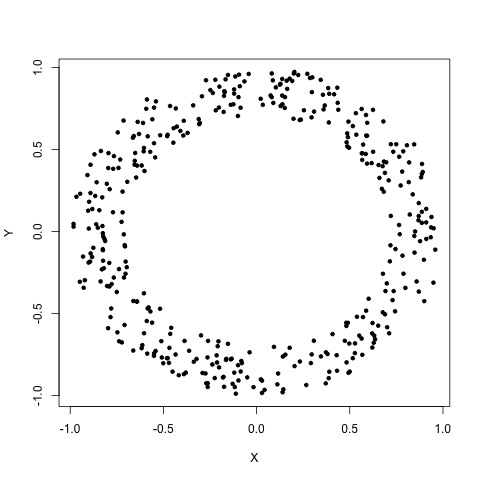
\includegraphics[height=7cm]{new-annulus.jpg}


\end{document}

